% Created by tikzDevice version 0.12.6 on 2024-10-23 19:35:46
% !TEX encoding = UTF-8 Unicode
\begin{tikzpicture}[x=1pt,y=1pt]
\definecolor{fillColor}{RGB}{255,255,255}
\path[use as bounding box,fill=fillColor,fill opacity=0.00] (0,0) rectangle (289.08,144.54);
\begin{scope}
\path[clip] (  0.00,  0.00) rectangle (289.08,144.54);
\definecolor{drawColor}{RGB}{255,255,255}
\definecolor{fillColor}{RGB}{255,255,255}

\path[draw=drawColor,line width= 0.6pt,line join=round,line cap=round,fill=fillColor] (  0.00,  0.00) rectangle (289.08,144.54);
\end{scope}
\begin{scope}
\path[clip] ( 36.11, 30.69) rectangle (283.58,139.04);
\definecolor{fillColor}{RGB}{255,255,255}

\path[fill=fillColor] ( 36.11, 30.69) rectangle (283.58,139.04);
\definecolor{drawColor}{gray}{0.92}

\path[draw=drawColor,line width= 0.3pt,line join=round] ( 36.11, 38.47) --
	(283.58, 38.47);

\path[draw=drawColor,line width= 0.3pt,line join=round] ( 36.11, 61.31) --
	(283.58, 61.31);

\path[draw=drawColor,line width= 0.3pt,line join=round] ( 36.11, 84.15) --
	(283.58, 84.15);

\path[draw=drawColor,line width= 0.3pt,line join=round] ( 36.11,107.00) --
	(283.58,107.00);

\path[draw=drawColor,line width= 0.3pt,line join=round] ( 36.11,129.84) --
	(283.58,129.84);

\path[draw=drawColor,line width= 0.3pt,line join=round] ( 69.86, 30.69) --
	( 69.86,139.04);

\path[draw=drawColor,line width= 0.3pt,line join=round] (144.85, 30.69) --
	(144.85,139.04);

\path[draw=drawColor,line width= 0.3pt,line join=round] (219.84, 30.69) --
	(219.84,139.04);

\path[draw=drawColor,line width= 0.6pt,line join=round] ( 36.11, 49.89) --
	(283.58, 49.89);

\path[draw=drawColor,line width= 0.6pt,line join=round] ( 36.11, 72.73) --
	(283.58, 72.73);

\path[draw=drawColor,line width= 0.6pt,line join=round] ( 36.11, 95.57) --
	(283.58, 95.57);

\path[draw=drawColor,line width= 0.6pt,line join=round] ( 36.11,118.42) --
	(283.58,118.42);

\path[draw=drawColor,line width= 0.6pt,line join=round] (107.35, 30.69) --
	(107.35,139.04);

\path[draw=drawColor,line width= 0.6pt,line join=round] (182.34, 30.69) --
	(182.34,139.04);

\path[draw=drawColor,line width= 0.6pt,line join=round] (257.33, 30.69) --
	(257.33,139.04);
\definecolor{drawColor}{RGB}{255,105,97}
\definecolor{fillColor}{RGB}{255,105,97}

\path[draw=drawColor,line width= 0.4pt,line join=round,line cap=round,fill=fillColor] (122.35, 70.76) circle (  1.96);

\path[draw=drawColor,line width= 0.4pt,line join=round,line cap=round,fill=fillColor] (152.35, 65.36) circle (  1.96);

\path[draw=drawColor,line width= 0.4pt,line join=round,line cap=round,fill=fillColor] ( 92.35, 71.51) circle (  1.96);

\path[draw=drawColor,line width= 0.4pt,line join=round,line cap=round,fill=fillColor] (152.35, 81.89) circle (  1.96);

\path[draw=drawColor,line width= 0.4pt,line join=round,line cap=round,fill=fillColor] ( 47.36, 94.26) circle (  1.96);

\path[draw=drawColor,line width= 0.4pt,line join=round,line cap=round,fill=fillColor] (167.34, 60.12) circle (  1.96);

\path[draw=drawColor,line width= 0.4pt,line join=round,line cap=round,fill=fillColor] ( 62.36, 89.14) circle (  1.96);

\path[draw=drawColor,line width= 0.4pt,line join=round,line cap=round,fill=fillColor] ( 92.35, 48.91) circle (  1.96);

\path[draw=drawColor,line width= 0.4pt,line join=round,line cap=round,fill=fillColor] (107.35, 61.41) circle (  1.96);

\path[draw=drawColor,line width= 0.4pt,line join=round,line cap=round,fill=fillColor] (129.85, 41.24) circle (  1.96);

\path[draw=drawColor,line width= 0.4pt,line join=round,line cap=round,fill=fillColor] ( 99.85, 69.95) circle (  1.96);

\path[draw=drawColor,line width= 0.4pt,line join=round,line cap=round,fill=fillColor] (107.35, 73.52) circle (  1.96);

\path[draw=drawColor,line width= 0.4pt,line join=round,line cap=round,fill=fillColor] ( 99.85, 80.40) circle (  1.96);

\path[draw=drawColor,line width= 0.4pt,line join=round,line cap=round,fill=fillColor] (137.35, 54.38) circle (  1.96);

\path[draw=drawColor,line width= 0.4pt,line join=round,line cap=round,fill=fillColor] (107.35, 77.80) circle (  1.96);

\path[draw=drawColor,line width= 0.4pt,line join=round,line cap=round,fill=fillColor] (107.35, 75.81) circle (  1.96);

\path[draw=drawColor,line width= 0.4pt,line join=round,line cap=round,fill=fillColor] (152.35, 50.49) circle (  1.96);

\path[draw=drawColor,line width= 0.4pt,line join=round,line cap=round,fill=fillColor] (122.35, 73.57) circle (  1.96);

\path[draw=drawColor,line width= 0.4pt,line join=round,line cap=round,fill=fillColor] (107.35, 64.51) circle (  1.96);

\path[draw=drawColor,line width= 0.4pt,line join=round,line cap=round,fill=fillColor] (159.85, 79.15) circle (  1.96);

\path[draw=drawColor,line width= 0.4pt,line join=round,line cap=round,fill=fillColor] ( 69.86, 78.13) circle (  1.96);

\path[draw=drawColor,line width= 0.4pt,line join=round,line cap=round,fill=fillColor] (144.85, 58.98) circle (  1.96);

\path[draw=drawColor,line width= 0.4pt,line join=round,line cap=round,fill=fillColor] (122.35, 56.92) circle (  1.96);

\path[draw=drawColor,line width= 0.4pt,line join=round,line cap=round,fill=fillColor] (114.85, 55.63) circle (  1.96);

\path[draw=drawColor,line width= 0.4pt,line join=round,line cap=round,fill=fillColor] ( 92.35, 61.94) circle (  1.96);

\path[draw=drawColor,line width= 0.4pt,line join=round,line cap=round,fill=fillColor] (137.35, 82.09) circle (  1.96);

\path[draw=drawColor,line width= 0.4pt,line join=round,line cap=round,fill=fillColor] (137.35, 73.50) circle (  1.96);

\path[draw=drawColor,line width= 0.4pt,line join=round,line cap=round,fill=fillColor] ( 92.35, 72.92) circle (  1.96);

\path[draw=drawColor,line width= 0.4pt,line join=round,line cap=round,fill=fillColor] (129.85, 44.75) circle (  1.96);

\path[draw=drawColor,line width= 0.4pt,line join=round,line cap=round,fill=fillColor] (122.35, 60.49) circle (  1.96);

\path[draw=drawColor,line width= 0.4pt,line join=round,line cap=round,fill=fillColor] ( 62.36, 84.70) circle (  1.96);

\path[draw=drawColor,line width= 0.4pt,line join=round,line cap=round,fill=fillColor] (122.35, 79.56) circle (  1.96);

\path[draw=drawColor,line width= 0.4pt,line join=round,line cap=round,fill=fillColor] ( 92.35, 70.46) circle (  1.96);

\path[draw=drawColor,line width= 0.4pt,line join=round,line cap=round,fill=fillColor] ( 92.35, 63.09) circle (  1.96);

\path[draw=drawColor,line width= 0.4pt,line join=round,line cap=round,fill=fillColor] (144.85, 72.72) circle (  1.96);

\path[draw=drawColor,line width= 0.4pt,line join=round,line cap=round,fill=fillColor] (114.85, 62.18) circle (  1.96);

\path[draw=drawColor,line width= 0.4pt,line join=round,line cap=round,fill=fillColor] ( 77.36, 75.35) circle (  1.96);

\path[draw=drawColor,line width= 0.4pt,line join=round,line cap=round,fill=fillColor] (107.35, 97.26) circle (  1.96);

\path[draw=drawColor,line width= 0.4pt,line join=round,line cap=round,fill=fillColor] ( 77.36, 67.60) circle (  1.96);

\path[draw=drawColor,line width= 0.4pt,line join=round,line cap=round,fill=fillColor] (114.85, 75.01) circle (  1.96);

\path[draw=drawColor,line width= 0.4pt,line join=round,line cap=round,fill=fillColor] (107.35, 56.04) circle (  1.96);

\path[draw=drawColor,line width= 0.4pt,line join=round,line cap=round,fill=fillColor] (129.85, 60.28) circle (  1.96);

\path[draw=drawColor,line width= 0.4pt,line join=round,line cap=round,fill=fillColor] ( 84.86, 83.59) circle (  1.96);

\path[draw=drawColor,line width= 0.4pt,line join=round,line cap=round,fill=fillColor] ( 84.86, 76.20) circle (  1.96);

\path[draw=drawColor,line width= 0.4pt,line join=round,line cap=round,fill=fillColor] ( 84.86, 69.32) circle (  1.96);

\path[draw=drawColor,line width= 0.4pt,line join=round,line cap=round,fill=fillColor] ( 99.85, 98.17) circle (  1.96);

\path[draw=drawColor,line width= 0.4pt,line join=round,line cap=round,fill=fillColor] (129.85, 35.61) circle (  1.96);

\path[draw=drawColor,line width= 0.4pt,line join=round,line cap=round,fill=fillColor] ( 84.86, 63.73) circle (  1.96);

\path[draw=drawColor,line width= 0.4pt,line join=round,line cap=round,fill=fillColor] ( 77.36, 66.97) circle (  1.96);

\path[draw=drawColor,line width= 0.4pt,line join=round,line cap=round,fill=fillColor] (129.85, 63.29) circle (  1.96);
\definecolor{drawColor}{RGB}{70,130,180}
\definecolor{fillColor}{RGB}{70,130,180}

\path[draw=drawColor,line width= 0.4pt,line join=round,line cap=round,fill=fillColor] (189.84, 85.00) circle (  1.96);

\path[draw=drawColor,line width= 0.4pt,line join=round,line cap=round,fill=fillColor] (272.33, 85.21) circle (  1.96);

\path[draw=drawColor,line width= 0.4pt,line join=round,line cap=round,fill=fillColor] (182.34, 87.64) circle (  1.96);

\path[draw=drawColor,line width= 0.4pt,line join=round,line cap=round,fill=fillColor] (189.84,107.36) circle (  1.96);

\path[draw=drawColor,line width= 0.4pt,line join=round,line cap=round,fill=fillColor] (234.84,103.55) circle (  1.96);

\path[draw=drawColor,line width= 0.4pt,line join=round,line cap=round,fill=fillColor] (174.84,118.82) circle (  1.96);

\path[draw=drawColor,line width= 0.4pt,line join=round,line cap=round,fill=fillColor] (167.34, 75.94) circle (  1.96);

\path[draw=drawColor,line width= 0.4pt,line join=round,line cap=round,fill=fillColor] (174.84, 94.66) circle (  1.96);

\path[draw=drawColor,line width= 0.4pt,line join=round,line cap=round,fill=fillColor] (204.84,111.28) circle (  1.96);

\path[draw=drawColor,line width= 0.4pt,line join=round,line cap=round,fill=fillColor] (182.34, 90.44) circle (  1.96);

\path[draw=drawColor,line width= 0.4pt,line join=round,line cap=round,fill=fillColor] (137.35,103.26) circle (  1.96);

\path[draw=drawColor,line width= 0.4pt,line join=round,line cap=round,fill=fillColor] (167.34,108.57) circle (  1.96);

\path[draw=drawColor,line width= 0.4pt,line join=round,line cap=round,fill=fillColor] (182.34,105.39) circle (  1.96);

\path[draw=drawColor,line width= 0.4pt,line join=round,line cap=round,fill=fillColor] (197.34,107.66) circle (  1.96);

\path[draw=drawColor,line width= 0.4pt,line join=round,line cap=round,fill=fillColor] (144.85,114.63) circle (  1.96);

\path[draw=drawColor,line width= 0.4pt,line join=round,line cap=round,fill=fillColor] (227.34, 84.55) circle (  1.96);

\path[draw=drawColor,line width= 0.4pt,line join=round,line cap=round,fill=fillColor] (204.84, 60.38) circle (  1.96);

\path[draw=drawColor,line width= 0.4pt,line join=round,line cap=round,fill=fillColor] (167.34,108.29) circle (  1.96);

\path[draw=drawColor,line width= 0.4pt,line join=round,line cap=round,fill=fillColor] (137.35,134.11) circle (  1.96);

\path[draw=drawColor,line width= 0.4pt,line join=round,line cap=round,fill=fillColor] (204.84, 94.89) circle (  1.96);

\path[draw=drawColor,line width= 0.4pt,line join=round,line cap=round,fill=fillColor] (189.84, 99.15) circle (  1.96);

\path[draw=drawColor,line width= 0.4pt,line join=round,line cap=round,fill=fillColor] (152.35,105.06) circle (  1.96);

\path[draw=drawColor,line width= 0.4pt,line join=round,line cap=round,fill=fillColor] (182.34, 91.08) circle (  1.96);

\path[draw=drawColor,line width= 0.4pt,line join=round,line cap=round,fill=fillColor] (137.35,121.31) circle (  1.96);

\path[draw=drawColor,line width= 0.4pt,line join=round,line cap=round,fill=fillColor] (137.35,126.91) circle (  1.96);

\path[draw=drawColor,line width= 0.4pt,line join=round,line cap=round,fill=fillColor] (189.84, 95.17) circle (  1.96);

\path[draw=drawColor,line width= 0.4pt,line join=round,line cap=round,fill=fillColor] (189.84, 91.90) circle (  1.96);

\path[draw=drawColor,line width= 0.4pt,line join=round,line cap=round,fill=fillColor] (144.85, 98.91) circle (  1.96);

\path[draw=drawColor,line width= 0.4pt,line join=round,line cap=round,fill=fillColor] (189.84,114.42) circle (  1.96);

\path[draw=drawColor,line width= 0.4pt,line join=round,line cap=round,fill=fillColor] (129.85,100.34) circle (  1.96);

\path[draw=drawColor,line width= 0.4pt,line join=round,line cap=round,fill=fillColor] (182.34, 91.54) circle (  1.96);

\path[draw=drawColor,line width= 0.4pt,line join=round,line cap=round,fill=fillColor] (182.34,113.71) circle (  1.96);

\path[draw=drawColor,line width= 0.4pt,line join=round,line cap=round,fill=fillColor] (249.83, 98.93) circle (  1.96);

\path[draw=drawColor,line width= 0.4pt,line join=round,line cap=round,fill=fillColor] (182.34, 96.16) circle (  1.96);

\path[draw=drawColor,line width= 0.4pt,line join=round,line cap=round,fill=fillColor] (167.34,129.67) circle (  1.96);

\path[draw=drawColor,line width= 0.4pt,line join=round,line cap=round,fill=fillColor] (189.84,113.48) circle (  1.96);

\path[draw=drawColor,line width= 0.4pt,line join=round,line cap=round,fill=fillColor] (212.34, 90.23) circle (  1.96);

\path[draw=drawColor,line width= 0.4pt,line join=round,line cap=round,fill=fillColor] (137.35, 96.53) circle (  1.96);

\path[draw=drawColor,line width= 0.4pt,line join=round,line cap=round,fill=fillColor] (152.35,104.38) circle (  1.96);

\path[draw=drawColor,line width= 0.4pt,line join=round,line cap=round,fill=fillColor] (189.84, 95.21) circle (  1.96);

\path[draw=drawColor,line width= 0.4pt,line join=round,line cap=round,fill=fillColor] (204.84, 96.80) circle (  1.96);

\path[draw=drawColor,line width= 0.4pt,line join=round,line cap=round,fill=fillColor] (144.85, 87.97) circle (  1.96);

\path[draw=drawColor,line width= 0.4pt,line join=round,line cap=round,fill=fillColor] (167.34, 90.09) circle (  1.96);

\path[draw=drawColor,line width= 0.4pt,line join=round,line cap=round,fill=fillColor] (212.34, 81.97) circle (  1.96);

\path[draw=drawColor,line width= 0.4pt,line join=round,line cap=round,fill=fillColor] (122.35,122.05) circle (  1.96);

\path[draw=drawColor,line width= 0.4pt,line join=round,line cap=round,fill=fillColor] (189.84, 93.92) circle (  1.96);

\path[draw=drawColor,line width= 0.4pt,line join=round,line cap=round,fill=fillColor] (189.84, 98.14) circle (  1.96);

\path[draw=drawColor,line width= 0.4pt,line join=round,line cap=round,fill=fillColor] (182.34, 90.96) circle (  1.96);

\path[draw=drawColor,line width= 0.4pt,line join=round,line cap=round,fill=fillColor] (197.34, 97.66) circle (  1.96);

\path[draw=drawColor,line width= 0.4pt,line join=round,line cap=round,fill=fillColor] (197.34, 84.55) circle (  1.96);
\definecolor{drawColor}{RGB}{255,105,97}

\path[draw=drawColor,line width= 1.1pt,line join=round] ( 47.36, 80.75) --
	( 48.88, 80.46) --
	( 50.40, 80.18) --
	( 51.92, 79.90) --
	( 53.43, 79.61) --
	( 54.95, 79.33) --
	( 56.47, 79.05) --
	( 57.99, 78.76) --
	( 59.51, 78.48) --
	( 61.03, 78.20) --
	( 62.55, 77.91) --
	( 64.07, 77.63) --
	( 65.59, 77.34) --
	( 67.10, 77.06) --
	( 68.62, 76.78) --
	( 70.14, 76.49) --
	( 71.66, 76.21) --
	( 73.18, 75.93) --
	( 74.70, 75.64) --
	( 76.22, 75.36) --
	( 77.74, 75.08) --
	( 79.25, 74.79) --
	( 80.77, 74.51) --
	( 82.29, 74.23) --
	( 83.81, 73.94) --
	( 85.33, 73.66) --
	( 86.85, 73.37) --
	( 88.37, 73.09) --
	( 89.89, 72.81) --
	( 91.40, 72.52) --
	( 92.92, 72.24) --
	( 94.44, 71.96) --
	( 95.96, 71.67) --
	( 97.48, 71.39) --
	( 99.00, 71.11) --
	(100.52, 70.82) --
	(102.04, 70.54) --
	(103.56, 70.25) --
	(105.07, 69.97) --
	(106.59, 69.69) --
	(108.11, 69.40) --
	(109.63, 69.12) --
	(111.15, 68.84) --
	(112.67, 68.55) --
	(114.19, 68.27) --
	(115.71, 67.99) --
	(117.22, 67.70) --
	(118.74, 67.42) --
	(120.26, 67.14) --
	(121.78, 66.85) --
	(123.30, 66.57) --
	(124.82, 66.28) --
	(126.34, 66.00) --
	(127.86, 65.72) --
	(129.37, 65.43) --
	(130.89, 65.15) --
	(132.41, 64.87) --
	(133.93, 64.58) --
	(135.45, 64.30) --
	(136.97, 64.02) --
	(138.49, 63.73) --
	(140.01, 63.45) --
	(141.53, 63.16) --
	(143.04, 62.88) --
	(144.56, 62.60) --
	(146.08, 62.31) --
	(147.60, 62.03) --
	(149.12, 61.75) --
	(150.64, 61.46) --
	(152.16, 61.18) --
	(153.68, 60.90) --
	(155.19, 60.61) --
	(156.71, 60.33) --
	(158.23, 60.05) --
	(159.75, 59.76) --
	(161.27, 59.48) --
	(162.79, 59.19) --
	(164.31, 58.91) --
	(165.83, 58.63) --
	(167.34, 58.34);
\definecolor{drawColor}{RGB}{70,130,180}

\path[draw=drawColor,line width= 1.1pt,line join=round] (122.35,111.96) --
	(124.25,111.57) --
	(126.15,111.19) --
	(128.05,110.80) --
	(129.94,110.41) --
	(131.84,110.02) --
	(133.74,109.63) --
	(135.64,109.24) --
	(137.54,108.86) --
	(139.44,108.47) --
	(141.34,108.08) --
	(143.23,107.69) --
	(145.13,107.30) --
	(147.03,106.91) --
	(148.93,106.53) --
	(150.83,106.14) --
	(152.73,105.75) --
	(154.62,105.36) --
	(156.52,104.97) --
	(158.42,104.58) --
	(160.32,104.19) --
	(162.22,103.81) --
	(164.12,103.42) --
	(166.02,103.03) --
	(167.91,102.64) --
	(169.81,102.25) --
	(171.71,101.86) --
	(173.61,101.48) --
	(175.51,101.09) --
	(177.41,100.70) --
	(179.31,100.31) --
	(181.20, 99.92) --
	(183.10, 99.53) --
	(185.00, 99.15) --
	(186.90, 98.76) --
	(188.80, 98.37) --
	(190.70, 97.98) --
	(192.59, 97.59) --
	(194.49, 97.20) --
	(196.39, 96.82) --
	(198.29, 96.43) --
	(200.19, 96.04) --
	(202.09, 95.65) --
	(203.99, 95.26) --
	(205.88, 94.87) --
	(207.78, 94.48) --
	(209.68, 94.10) --
	(211.58, 93.71) --
	(213.48, 93.32) --
	(215.38, 92.93) --
	(217.28, 92.54) --
	(219.17, 92.15) --
	(221.07, 91.77) --
	(222.97, 91.38) --
	(224.87, 90.99) --
	(226.77, 90.60) --
	(228.67, 90.21) --
	(230.56, 89.82) --
	(232.46, 89.44) --
	(234.36, 89.05) --
	(236.26, 88.66) --
	(238.16, 88.27) --
	(240.06, 87.88) --
	(241.96, 87.49) --
	(243.85, 87.11) --
	(245.75, 86.72) --
	(247.65, 86.33) --
	(249.55, 85.94) --
	(251.45, 85.55) --
	(253.35, 85.16) --
	(255.24, 84.77) --
	(257.14, 84.39) --
	(259.04, 84.00) --
	(260.94, 83.61) --
	(262.84, 83.22) --
	(264.74, 82.83) --
	(266.64, 82.44) --
	(268.53, 82.06) --
	(270.43, 81.67) --
	(272.33, 81.28);
\definecolor{drawColor}{gray}{0.20}

\path[draw=drawColor,line width= 0.6pt,line join=round,line cap=round] ( 36.11, 30.69) rectangle (283.58,139.04);
\end{scope}
\begin{scope}
\path[clip] (  0.00,  0.00) rectangle (289.08,144.54);
\definecolor{drawColor}{gray}{0.30}

\node[text=drawColor,anchor=base east,inner sep=0pt, outer sep=0pt, scale=  0.88] at ( 31.16, 46.86) {75};

\node[text=drawColor,anchor=base east,inner sep=0pt, outer sep=0pt, scale=  0.88] at ( 31.16, 69.70) {100};

\node[text=drawColor,anchor=base east,inner sep=0pt, outer sep=0pt, scale=  0.88] at ( 31.16, 92.54) {125};

\node[text=drawColor,anchor=base east,inner sep=0pt, outer sep=0pt, scale=  0.88] at ( 31.16,115.39) {150};
\end{scope}
\begin{scope}
\path[clip] (  0.00,  0.00) rectangle (289.08,144.54);
\definecolor{drawColor}{gray}{0.20}

\path[draw=drawColor,line width= 0.6pt,line join=round] ( 33.36, 49.89) --
	( 36.11, 49.89);

\path[draw=drawColor,line width= 0.6pt,line join=round] ( 33.36, 72.73) --
	( 36.11, 72.73);

\path[draw=drawColor,line width= 0.6pt,line join=round] ( 33.36, 95.57) --
	( 36.11, 95.57);

\path[draw=drawColor,line width= 0.6pt,line join=round] ( 33.36,118.42) --
	( 36.11,118.42);
\end{scope}
\begin{scope}
\path[clip] (  0.00,  0.00) rectangle (289.08,144.54);
\definecolor{drawColor}{gray}{0.20}

\path[draw=drawColor,line width= 0.6pt,line join=round] (107.35, 27.94) --
	(107.35, 30.69);

\path[draw=drawColor,line width= 0.6pt,line join=round] (182.34, 27.94) --
	(182.34, 30.69);

\path[draw=drawColor,line width= 0.6pt,line join=round] (257.33, 27.94) --
	(257.33, 30.69);
\end{scope}
\begin{scope}
\path[clip] (  0.00,  0.00) rectangle (289.08,144.54);
\definecolor{drawColor}{gray}{0.30}

\node[text=drawColor,anchor=base,inner sep=0pt, outer sep=0pt, scale=  0.88] at (107.35, 19.68) {10};

\node[text=drawColor,anchor=base,inner sep=0pt, outer sep=0pt, scale=  0.88] at (182.34, 19.68) {20};

\node[text=drawColor,anchor=base,inner sep=0pt, outer sep=0pt, scale=  0.88] at (257.33, 19.68) {30};
\end{scope}
\begin{scope}
\path[clip] (  0.00,  0.00) rectangle (289.08,144.54);
\definecolor{drawColor}{RGB}{0,0,0}

\node[text=drawColor,anchor=base,inner sep=0pt, outer sep=0pt, scale=  1.10] at (159.85,  7.64) {Number of cigarettes smoked per week};
\end{scope}
\begin{scope}
\path[clip] (  0.00,  0.00) rectangle (289.08,144.54);
\definecolor{drawColor}{RGB}{0,0,0}

\node[text=drawColor,rotate= 90.00,anchor=base,inner sep=0pt, outer sep=0pt, scale=  1.10] at ( 13.08, 84.86) {Sport performance};
\end{scope}
\begin{scope}
\path[clip] (  0.00,  0.00) rectangle (289.08,144.54);
\definecolor{fillColor}{RGB}{255,255,255}

\path[fill=fillColor] (222.24, 31.32) rectangle (283.06, 71.23);
\end{scope}
\begin{scope}
\path[clip] (  0.00,  0.00) rectangle (289.08,144.54);
\definecolor{fillColor}{RGB}{255,255,255}

\path[fill=fillColor] (227.74, 51.27) rectangle (242.19, 65.73);
\end{scope}
\begin{scope}
\path[clip] (  0.00,  0.00) rectangle (289.08,144.54);
\definecolor{drawColor}{RGB}{255,105,97}
\definecolor{fillColor}{RGB}{255,105,97}

\path[draw=drawColor,line width= 0.4pt,line join=round,line cap=round,fill=fillColor] (234.96, 58.50) circle (  1.96);
\end{scope}
\begin{scope}
\path[clip] (  0.00,  0.00) rectangle (289.08,144.54);
\definecolor{drawColor}{RGB}{255,105,97}

\path[draw=drawColor,line width= 1.1pt,line join=round] (229.18, 58.50) -- (240.75, 58.50);
\end{scope}
\begin{scope}
\path[clip] (  0.00,  0.00) rectangle (289.08,144.54);
\definecolor{fillColor}{RGB}{255,255,255}

\path[fill=fillColor] (227.74, 36.82) rectangle (242.19, 51.27);
\end{scope}
\begin{scope}
\path[clip] (  0.00,  0.00) rectangle (289.08,144.54);
\definecolor{drawColor}{RGB}{70,130,180}
\definecolor{fillColor}{RGB}{70,130,180}

\path[draw=drawColor,line width= 0.4pt,line join=round,line cap=round,fill=fillColor] (234.96, 44.05) circle (  1.96);
\end{scope}
\begin{scope}
\path[clip] (  0.00,  0.00) rectangle (289.08,144.54);
\definecolor{drawColor}{RGB}{70,130,180}

\path[draw=drawColor,line width= 1.1pt,line join=round] (229.18, 44.05) -- (240.75, 44.05);
\end{scope}
\begin{scope}
\path[clip] (  0.00,  0.00) rectangle (289.08,144.54);
\definecolor{drawColor}{RGB}{0,0,0}

\node[text=drawColor,anchor=base west,inner sep=0pt, outer sep=0pt, scale=  0.88] at (247.69, 55.47) {\faVenus};
\end{scope}
\begin{scope}
\path[clip] (  0.00,  0.00) rectangle (289.08,144.54);
\definecolor{drawColor}{RGB}{0,0,0}

\node[text=drawColor,anchor=base west,inner sep=0pt, outer sep=0pt, scale=  0.88] at (247.69, 41.02) {\faMars};
\end{scope}
\end{tikzpicture}
